\subsection{Theoretical graph of the molar mass versus conversion}

    \begin{figure}[H]
        \centering
        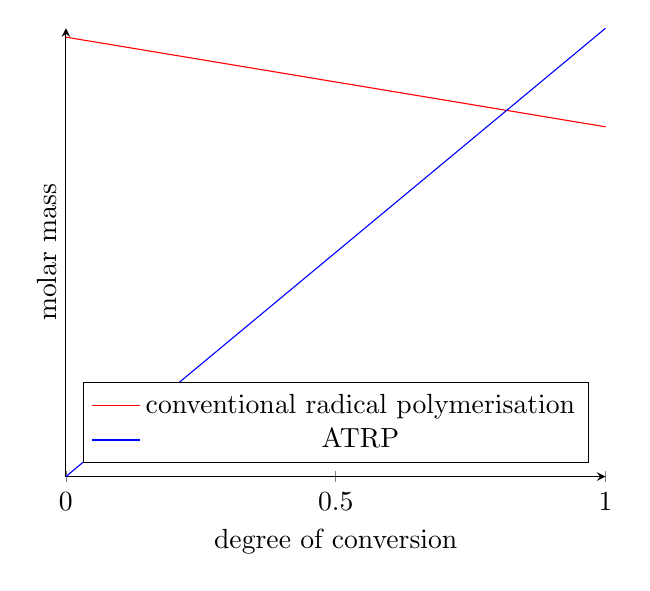
\begin{tikzpicture}
            \begin{axis}[
                ymajorticks=false,
                xtick={0,0.5,1},
                axis lines = left,
                xlabel = degree of conversion,
                ylabel = molar mass,
                legend pos=south east,
            ]
            %Below the red parabola is defined
            \addplot [
                domain=-0:1, 
                samples=10, 
                color=red,
            ]
            {0.98-0.2*x};
            \addlegendentry{conventional radical polymerisation}
            %Here the blue parabola is defined
            \addplot [
                domain=-0:1, 
                samples=10, 
                color=blue,
                ]
                {x};
            \addlegendentry{ATRP}
            
            \end{axis}
            \end{tikzpicture}
            \caption{Theoretical graph}  
    \end{figure}

For the conventional radical polymerisation high molar masses are acquired very 
early in the reaction and due to termination reactions the average molar mass decreases 
for increasing conversion. The ATRP method on the other hand yields a linear relation between the molar mass 
and conversion due to it's controlled nature where the polymer ends can react until all of the monomer has 
been consumed.z

    